\chapter{Graph Theory}
\label{ch:bg::graphs}

\begin{cluster}
\label{grp:prmbl:bg::graphs::presents}

\begin{preamble}
\label{prmbl:bg::graphs::presents}
This chapter presents an overview of basic graph theory
used throughout the book.
This chapter does not aim to be complete (and is far from it) but
tries to cover the most relevant material to the course.  
More details can be found in standard texts.

\end{preamble}
\end{cluster}


\section{Basic Definitions}
\label{sec:bg::graphs::basics}

\begin{cluster}
\label{grp:tch:bg::graphs::todo}

\begin{teachnote}
\label{tch:bg::graphs::todo}
TODO

Hamiltonian paths/cycles.

Define Diameter

\end{teachnote}
\end{cluster}

\begin{cluster}
\label{grp:def:bg::graphs::directed-graph}

\begin{definition}[Directed Graph]
\label{def:bg::graphs::directed-graph}
A~\defn{directed graph}~or (\defn{digraph})~is a pair $G = (V,A)$
where
\begin{itemize}
\item $V$ is a set of~\defn{vertices},~and

\item $A \subseteq V \times V$ is a set of~\defn{directed edges}~or \defn{arcs}.
\end{itemize}

\end{definition}
\end{cluster}

\begin{cluster}
\label{grp:nt:bg::graphs::digraph}

\begin{note}
\label{nt:bg::graphs::digraph}
In a digraph, each arc is an ordered pair $e = (u,v)$.  A digraph can
have~\defn{self loops}~$(u,u)$.  

\end{note}
\end{cluster}

\begin{cluster}
\label{grp:def:bg::graphs::undirected-graph}

\begin{definition}[Undirected graph]
\label{def:bg::graphs::undirected-graph}
 An~\defn{undirected graph}~is a pair $G = (V,E)$ where
\begin{itemize}
\item  $V$ is a set of~\defn{vertices}~(or nodes), and
\item  $E \subseteq  \binom{V}{2}$ is a set of edges.
\end{itemize}

\end{definition}
\end{cluster}

\begin{cluster}
\label{grp:nt:bg::graphs::given}

\begin{note}
\label{nt:bg::graphs::given}
Given a set $V$, a~\defn{k-combination}~of~$V$ is a subset of
$k$~distinct elements of~$V$.
The notation 
\[
\binom{V}{k}
\]
denotes the set of all $k$-combinations of the set~$V$. 

Therefore, in an undirected graph, each edge is an unordered pair
$e = \{ u,v \}$ (or equivalently $\{ v,u \}$)
and there cannot be self loops ($\{v,v\} = \{v\} \not\in
\binom{V}{2}$).

\end{note}
\end{cluster}

\begin{cluster}
\label{grp:ex:bg::graphs::basics::examples}

\begin{example}
\label{ex:bg::graphs::basics::examples}
An example directed graph with $4$ vertices:

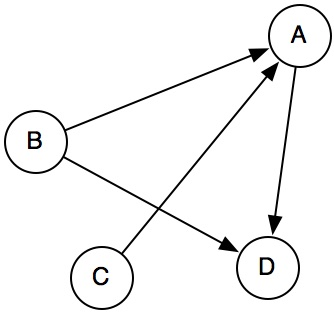
\includegraphics[width=2in]{background/media-graphs/directed1.jpg} 

An undirected graph on $4$ vertices, representing the
  K\"onigsberg problem. (Picture Source: Wikipedia):

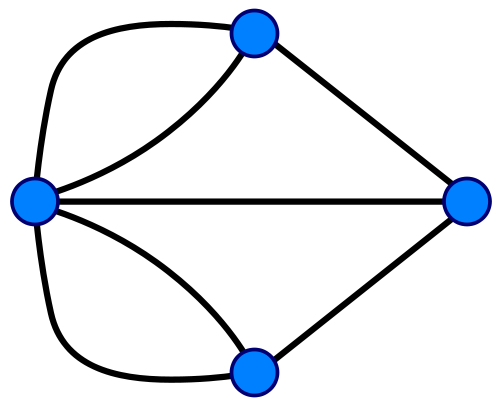
\includegraphics[width=2in]{background/media-graphs/konig.jpg}

\end{example}
\end{cluster}

\begin{cluster}
\label{grp:rmrk:bg::graphs::directed}

\begin{remark}
\label{rmrk:bg::graphs::directed}
While directed graphs represent possibly asymmetric relationships,
undirected graphs represent symmetric relationships.
Directed graphs are therefore more general than undirected graphs
because an undirected graph can be represented by a directed graph by
replacing an edge with two arcs, one in each direction.

\end{remark}
\end{cluster}

\begin{cluster}
\label{grp:grm:bg::graphs::graphs}

\begin{gram}
\label{grm:bg::graphs::graphs}
Graphs come with a lot of terminology, but fortunately most of it is
intuitive once we understand the concept.  
In this section, we consider graphs that do not have any data
associated with edges, such as weights.
In the next section, we consider weighted graphs, where the weights on
edges can represent a distance, a capacity or the strength of the
connection.

\end{gram}
\end{cluster}

\begin{cluster}
\label{grp:def:bg::graphs::neighbors}

\begin{definition}[Neighbors]
\label{def:bg::graphs::neighbors}
 A vertex $u$ is a~\defn{neighbor}~of, or
 equivalently~\defn{adjacent}~to, a vertex $v$ in a graph $G = (V,E)$
 if there is an edge $\{u,v\} \in E$.  For a directed graph a vertex
 $u$ is an~\defn{in-neighbor}~of a vertex $v$ if $(u,v) \in E$ and
 an~\defn{out-neighbor}~if $(v,u) \in E$.  We also say two edges or
 arcs are neighbors if they share a vertex.

\end{definition}
\end{cluster}

\begin{cluster}
\label{grp:def:bg::graphs::neighborhood}

\begin{definition}[Neighborhood]
\label{def:bg::graphs::neighborhood}
For an undirected graph $G = (V,E)$, the~\defn{neighborhood}~$N_G(v)$ 
of a vertex $v \in V$ is its set of all neighbors of $v$, i.e.,
$N_G(v) = \csetf{u}{\{u,v\} \in E}$. 
For a directed graph we use $N_G^+(v)$ to indicate the set of 
out-neighbors and $N_G^-(v)$ to indicate the set of in-neighbors of
$v$.  If we use $N_G(v)$ for a directed graph, we mean the out 
neighbors.  

The neighborhood of a set of vertices $U \subseteq V$ is the union of
their neighborhoods, e.g.,

\begin{itemize}
\item  $N_G(U) = \bigcup_{u \in U} N_G(y)$, or
\item $N_G^+(U) = \bigcup_{u \in U} N_G^+(u)$.
\end{itemize}

\end{definition}
\end{cluster}

\begin{cluster}
\label{grp:def:bg::graphs::incidence}

\begin{definition}[Incidence]
\label{def:bg::graphs::incidence}
We say an edge is~\defn{incident}~on a vertex if the vertex is one of
its endpoints.  Similarly we say a vertex is incident on an edge if it
is one of the endpoints of the edge.

\end{definition}
\end{cluster}

\begin{cluster}
\label{grp:def:bg::graphs::degree}

\begin{definition}[Degree]
\label{def:bg::graphs::degree}
 The~\defn{degree}~$d_G(v)$ of a vertex $v \in V$ in a graph $G =
 (V,E)$ is the size of the neighborhood $|N_G(v)|$.  For directed
 graphs we use~\defn{in-degree}~$d_G^-(v) = |N_G^-(v)|$
 and~\defn{out-degree}~$d_G^+(v) = |N_G^+(v)|$.  We will drop the
 subscript $G$ when it is clear from the context which graph we're
 talking about.

\end{definition}
\end{cluster}

\begin{cluster}
\label{grp:def:bg::graphs::path}

\begin{definition}[Path]
\label{def:bg::graphs::path}
A~\defn{path}~in a graph is a sequence of adjacent vertices.  
More formally for a graph $G = (V,E)$, we define the set of all paths
in $G$, written $\textit{Paths}(G)$ as 
\[
\textit{Paths}(G) = \csetf{P
  \in V^+}{1 \leq i < |P|, (P_i, P_{i+1}) \in E},
\]
where $V^+$ indicates all positive length sequences of vertices
(allowing for repeats).
The length of a path is one less than the number of vertices in the
path---i.e., it is the number of edges in the path.  A path in a
finite graph can have infinite length.  A~\defn{simple path}~is a path
with no repeated vertices.  Please see the remark below, however.

\end{definition}
\end{cluster}

\begin{cluster}
\label{grp:rmrk:bg::graphs::authors}

\begin{remark}
\label{rmrk:bg::graphs::authors}
Some authors use the terms walk for path, and path for
simple path.   Even in this book when it is clear from the context
we will sometimes drop the ``simple'' from simple path.

\end{remark}
\end{cluster}

\begin{cluster}
\label{grp:def:bg::graphs::reachability-and-connectivity}

\begin{definition}[Reachability and connectivity]
\label{def:bg::graphs::reachability-and-connectivity}
In a graph $G$, a vertex $u$ can~\defn{reach}~another vertex $v$
if there is a path in $G$ that starts at $u$ and ends at $v$.
If $u$ can reach $v$, we also say that $v$ is~\defn{reachable}~from $u$.
We use $R_G(u)$ to indicate the set of all vertices reachable from $u$
in $G$.
Note that in an undirected graph reachability is symmetric: if $u$ can reach $v$, then $v$ can reach $u$.

We say that an undirected graph is~\defn{connected}~if all vertices are reachable from all other vertices.  
We say that a directed graph is~\defn{strongly   connected}~if all vertices are reachable from all other vertices.

\end{definition}
\end{cluster}

\begin{cluster}
\label{grp:def:bg::graphs::cycles}

\begin{definition}[Cycles]
\label{def:bg::graphs::cycles}
In a directed graph a~\defn{cycle}~is a path that starts and ends at
the same vertex.    A cycle can have length one (i.e. a~\defn{self loop}).
A~\defn{simple cycle}~is a
cycle that has no repeated vertices other than the start and end
vertices being the same.
In an undirected graph a simple~\defn{cycle}~is a path that
starts and ends at the same vertex, has no repeated vertices other
than the first and last, and has length at least three.
In this course we will exclusively talk
about simple cycles and hence, as with paths, we will often drop
simple.

\end{definition}
\end{cluster}

\begin{cluster}
\label{grp:xrcs:bg::graphs::undirected}

\begin{exercise}
\label{xrcs:bg::graphs::undirected}
Why is important in a undirected graph to require that a cycle has
length at least three?  Why is important that we do not allow repeated
vertices?

\end{exercise}
\end{cluster}

\begin{cluster}
\label{grp:def:bg::graphs::trees-and-forests}

\begin{definition}[Trees and forests]
\label{def:bg::graphs::trees-and-forests}
An undirected graph with no cycles is a~\defn{forest}.
A forest that is connected is a~\defn{tree}.  
A directed graph is a forest (or tree) if when all edges are converted
to undirected edges it is undirected forest (or tree).  
A~\defn{rooted tree}~is a tree with one vertex designated as the root.
For a directed graph the edges are typically all directed toward the
root or away from the root.

\end{definition}
\end{cluster}

\begin{cluster}
\label{grp:def:bg::graphs::directed-acyclic-graphs}

\begin{definition}[Directed acyclic graphs]
\label{def:bg::graphs::directed-acyclic-graphs}
A directed graph with no cycles is a~\defn{directed acyclic graph}~(DAG).

\end{definition}
\end{cluster}

\begin{cluster}
\label{grp:def:bg::graphs::distance}

\begin{definition}[Distance]
\label{def:bg::graphs::distance}
The~\defn{distance}~$\delta_G(u,v)$ from a vertex $u$ to a vertex $v$
in a graph $G$ is the shortest path (minimum number of edges) from $u$
to $v$.  It is also referred to as the~\defn{shortest path
  length}~from $u$ to $v$.

\end{definition}
\end{cluster}

\begin{cluster}
\label{grp:def:bg::graphs::diameter}

\begin{definition}[Diameter]
\label{def:bg::graphs::diameter}
The~\defn{diameter}~of a graph $G$ is the maximum shortest path length over all
pairs of vertices in $G$, i.e., $\max\cset{\delta_G(u,v) : u, v \in V}$.

\end{definition}
\end{cluster}

\begin{cluster}
\label{grp:def:bg::graphs::multigraphs}

\begin{definition}[Multigraphs]
\label{def:bg::graphs::multigraphs}
Sometimes graphs allow multiple edges between the same pair of
vertices, called~\defn{multi-edges}.  Graphs with multi-edges are
called~\defn{multi-graphs}.  We will allow multi-edges in a couple
algorithms just for convenience.

\end{definition}
\end{cluster}

\begin{cluster}
\label{grp:def:bg::graphs::sparse-and-dense-graphs}

\begin{definition}[Sparse and Dense Graphs]
\label{def:bg::graphs::sparse-and-dense-graphs}
We will use the following conventions:
\begin{eqnarray*}
n & = |V|\\
m & = |E|
\end{eqnarray*}
Note that a directed graph can have at most $n^2$ edges (including self loops)
and an undirected graph at most $n(n-1)/2$.  We informally say that a graph
is~\defn{sparse}~if $m \ll n^2$ and~\defn{dense}~otherwise.  In most
applications graphs are very sparse, often with only a handful of neighbors per
vertex when averaged across vertices, although some vertices could have high
degree.  Therefore, the emphasis in the design of graph algorithms, at least for
this book, is on algorithms that work well for sparse graphs.

\end{definition}
\end{cluster}

\begin{cluster}
\label{grp:def:bg::graphs::basics::enumerable}

\begin{definition}[Enumerable graphs]
\label{def:bg::graphs::basics::enumerable}
In some cases, it is possible to label the vertices of the graphs with
natural numbers starting from $0$.  More precisely, an~\defn{enumerable graph} is a graph $G = (V,E)$ where $V =
\{0,1,\ldots,n-1\}$.
Enumerable graphs can be more efficient to represent than
general graphs.

\end{definition}
\end{cluster}


\section{Weighted Graphs}
\label{sec:bg::graphs::weighted}

\begin{cluster}
\label{grp:grm:bg::graphs::applications}

\begin{gram}
\label{grm:bg::graphs::applications}
\label{sec:bg::graphs::weighted}
\begin{gram}
Many applications of graphs require associating weights or other
values with the edges of a graph.  
\end{gram}

\end{gram}
\end{cluster}

\begin{cluster}
\label{grp:def:bg::graphs::weighted}

\begin{definition}[Weighted and Edge-Labeled Graphs]
\label{def:bg::graphs::weighted}
An \defn{edge-labeled graph}~or a \defn{weighted graph}~is a triple
$G = (E,V,w)$ where $w\!: E \to L$ is a function mapping edges or
directed edges to their labels (weights) , and $L$ is the set of
possible labels (weights).

\end{definition}
\end{cluster}

\begin{cluster}
\label{grp:grm:bg::graphs::graph}

\begin{gram}
\label{grm:bg::graphs::graph}
In a graph, if the data associated with the edges are real numbers, we
often use the term ``weight'' to refer to the edge labels, and use the
term ``weighted graph'' to refer to the graph.  In the general case,
we use the terms ``edge label'' and edge-labeled graph.  Weights or
other values on edges could represent many things, such as a distance,
or a capacity, or the strength of a relationship.

\end{gram}
\end{cluster}

\begin{cluster}
\label{grp:xmpl:bg::graphs::directed}

\begin{example}
\label{xmpl:bg::graphs::directed}
An example directed weighted graph.

\begin{center}
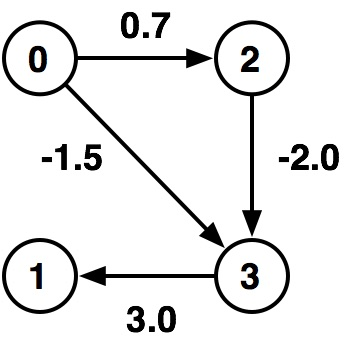
\includegraphics[width=1.5in]{background/media-graphs/dir-graph1.jpg}
\end{center}

\end{example}
\end{cluster}

\begin{cluster}
\label{grp:rmrk:bg::graphs::expected}

\begin{remark}
\label{rmrk:bg::graphs::expected}
As it may be expected, basic terminology on graphs defined above
straightforwardly extend to weighted graphs.

\end{remark}
\end{cluster}


\section{Subgraphs}
\label{sec:bg::graphs::subgraphs}

\begin{cluster}
\label{grp:grm:bg::graphs::working}

\begin{gram}
\label{grm:bg::graphs::working}
When working with graphs, we sometimes wish to refer to parts of a
graph.  To this end, we can use the notion of a subgraph, which refers
to a graph contained in a larger graph. A subgraph can be defined as
any subsets of edges and vertices that together constitute a well
defined graph.

\end{gram}
\end{cluster}

\begin{cluster}
\label{grp:def:bg::graphs::subgraph}

\begin{definition}[Subgraph]
\label{def:bg::graphs::subgraph}
Let $G = (V,E)$ and $H = (V', E')$ be two graphs.  $H$ is a
subgraph of if $V' \subseteq V$ and $E' \subseteq E$.

\end{definition}
\end{cluster}

\begin{cluster}
\label{grp:nt:bg::graphs::graph}

\begin{note}
\label{nt:bg::graphs::graph}
Note that since $H$ is a graph, the vertices defining each edge are in
the vertex set $V'$, i.e., for an undirected graph $E' \subseteq
\binom{V'}{2}$.  There are many possible subgraphs of a graph.

\end{note}
\end{cluster}

\begin{cluster}
\label{grp:grm:bg::graphs::class}

\begin{gram}
\label{grm:bg::graphs::class}
An important class of subgraphs are~\defn{vertex-induced subgraphs},
which are maximal subgraphs defined by a set of vertices.
A vertex-induced subgraph is maximal in the sense that it contains all
the edges that it can possibly contain.
In general when an object is said to be a~\defn{maximal}~``X'', it
means that nothing more can be added to the object without violating
the property ``X''.

\end{gram}
\end{cluster}

\begin{cluster}
\label{grp:def:bg::graphs::subgraph::vi}

\begin{definition}[Vertex-Induced Subgraph]
\label{def:bg::graphs::subgraph::vi}
The subgraph of $G = (V,E)$ induced by $V' \subseteq V$ is the graph $H
= (V',E')$ where $E' = \csetf{\cset{u,v} \in E}{u \in V', v \in V'}$.

\end{definition}
\end{cluster}

\begin{cluster}
\label{grp:xmpl:bg::graphs::vertex}

\begin{example}
\label{xmpl:bg::graphs::vertex}
Some vertex induced subgraphs:
\begin{center}
\begin{tabular}{c}
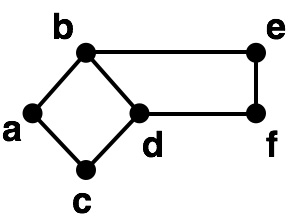
\includegraphics[width=2in]{background/media-graphs/contract-example1.jpg}
\\
Original graph 
\\
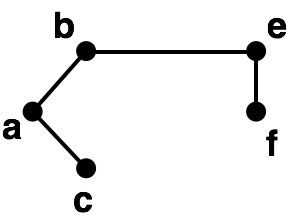
\includegraphics[width=2in]{background/media-graphs/induced-example.jpg}
\\
 Induced by
$\cset{\vname{a},\vname{b},\vname{c},\vname{e},\vname{f}}$ 
\\
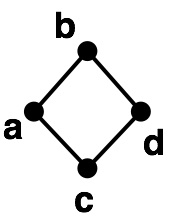
\includegraphics[width=1in]{background/media-graphs/induced-example2.jpg}
\\
Induced by $\cset{\vname{a},\vname{b},\vname{c},\vname{d}}$
\end{tabular}
\end{center}

\end{example}
\end{cluster}

\begin{cluster}
\label{grp:grm:bg::graphs::although}

\begin{gram}
\label{grm:bg::graphs::although}
Although we will not use it in this book, it is also possible to
define an induced subgraph in terms of a set of edges by including in
the graph all the vertices incident on the edges.

\end{gram}
\end{cluster}

\begin{cluster}
\label{grp:def:bg::graphs::subgraph::ei}

\begin{definition}[Edge-Induced Subgraph]
\label{def:bg::graphs::subgraph::ei}
The subgraph of $G = (V,E)$ induced by $E' \subseteq E$ is a graph $H
= (V',E')$ where $V' = \cup_{e \in E} e$.

\end{definition}
\end{cluster}


\section{Connectivity}
\label{sec:bg::graphs::connectivity}

\begin{cluster}
\label{grp:grm:bg::graphs::recall}

\begin{gram}
\label{grm:bg::graphs::recall}
Recall that in a graph (either directed or undirected) a vertex $v$ is
reachable from a vertex $u$ if there is a path from $u$ to $v$.  Also
recall that an undirected graph is connected if all vertices are
reachable from all other vertices. 

\end{gram}
\end{cluster}

\begin{cluster}
\label{grp:ex:gc-two-graphs}

\begin{example}
\label{ex:gc-two-graphs}
Two example graphs shown. The first in connected; the second is not.

\begin{tabular}{c}
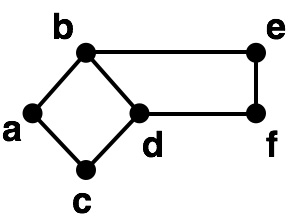
\includegraphics[width=2in]{background/media-graphs/contract-example1.jpg}
\\
{Graph 1}
\\
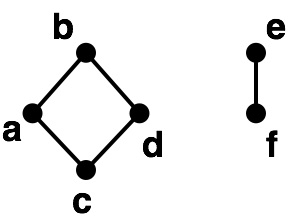
\includegraphics[width=2in]{background/media-graphs/contract-example4.jpg}
\\
{Graph 2}
\end{tabular}

An important subgraph of an undirected graph is a connected component
of a graph, defined below.

\end{example}
\end{cluster}

\begin{cluster}
\label{grp:def:bg::graphs::cc}

\begin{definition}[Connected Component]
\label{def:bg::graphs::cc}
Let $G = (V,E)$ be an undirected graph.  A subgraph $H$ of $G$ is
a~\defn{connected component}~of $G$ if it is a maximally connected
subgraph of $G$.

\end{definition}
\end{cluster}

\begin{cluster}
\label{grp:grm:bg::graphs::maximally}

\begin{gram}
\label{grm:bg::graphs::maximally}
Here, ``maximally connected component'' means we cannot add any more
vertices and edges from $G$ to $H$ without disconnecting $H$. In the
graphs shown in the example above, the first graph has one connected
component (hence it is connected); the second has two connected
components.

\end{gram}
\end{cluster}

\begin{cluster}
\label{grp:nt:bg::graphs::specify}

\begin{note}
\label{nt:bg::graphs::specify}
We can specify a connected component of a graph by simply specifying the
vertices in the component.
For example, the connected components of the second graph in the
example above can be specified as
$\cset{\vname{a},\vname{b},\vname{c},\vname{d}}$
and 
$\cset{\vname{e},\vname{f}}$.

\end{note}
\end{cluster}


\section{Graph Partition}
\label{sec:bg::graphs::partition}

\begin{cluster}
\label{grp:grm:bg::graphs::partition}

\begin{gram}
\label{grm:bg::graphs::partition}
Recall that a partition of a set $A$ is a set $P$ of non-empty subsets
of $A$ such that each element of $A$ is in exactly one subset, also
called block, $B \in P$.

\end{gram}
\end{cluster}

\begin{cluster}
\label{grp:def:bg::graphs::partition}

\begin{definition}[Graph Partition]
\label{def:bg::graphs::partition}
A~\defn{graph partition}~is a partition of the vertex set of the
graph.
More precisely, given graph $G = (V,E)$, we define a partition of $G$
as a set of graphs 
\[
P = \{ G_1 = (V_1,E_1) \ldots G_k = (V_k,E_k) \},
\]
where $\{V_1, \ldots, V_k\}$ is a (set) partition of $V$ and $G_1,
\ldots, G_k$ are vertex-induced subgraphs of $G$ with respect to $V_1,
\ldots, V_k$ respectively.  
As in set partitions, we use the term~\defn{part}~or~\defn{block}~to
refer to each vertex-induced subgraph $G_1, \ldots, G_k$.

\end{definition}
\end{cluster}

\begin{cluster}
\label{grp:def:bg::graphs::partition::edges}

\begin{definition}[Internal and Cut Edges]
\label{def:bg::graphs::partition::edges}
In a graph partition, we can distinguish between two kinds of edges:
internal edges and cut edges. ~\defn{Internal edges}~are edges that
are within a block;~\defn{cut edges}~are edges that are between
blocks.
One way to partition a graph is to make each connected component a
block. In such a partition, there are no cut edges between the
partitions.

\end{definition}
\end{cluster}


\section{Trees}
\label{sec:bg::graphs::trees}

\begin{cluster}
\label{grp:def:bg::graphs::tree}

\begin{definition}[Tree]
\label{def:bg::graphs::tree}
An undirected graph is a~\defn{tree}~if it does not have cycles and it is
connected.  A~\defn{rooted tree}~is a tree with a distinguished root
node that can be used to access all other nodes.
An example of a rooted tree along with
the associated terminology is given in below.

\end{definition}
\end{cluster}

\begin{cluster}
\label{grp:def:bg::graphs::rooted-tree}

\begin{definition}[Rooted Trees]
\label{def:bg::graphs::rooted-tree}

A~\defn{rooted tree}~is a directed graph such that
\begin{enumerate}
\item 
One of the vertices is the~\defn{root}~and it has no in edges.
\item 
All other vertices have one in-edge.
\item
There is a path from the root to all other vertices.
\end{enumerate}

Rooted trees are common structures in computing and have their own
dedicated terminology.
\begin{itemize}
\item
By convention we use the term~\defn{node}~instead of vertex to refer
to the vertices of a rooted tree.  
\item
A node is a~\defn{leaf}~if it has no out edges, and an~\defn{internal
  node}~otherwise.  

\item
For each directed edge $(u,v)$, $u$ is the~\defn{parent}~of $v$, and
$v$ is a~\defn{child}~of $u$.  

\item
For each path from $u$ to $v$ (including the empty path with $u = v$),
$u$ is an~\defn{ancestor}~of $v$, and $v$ is a~\defn{descendant}~of
$u$.
\item
For a vertex $v$, its~\defn{depth}~is the length of the path from the
root to $v$ and its~\defn{height}~is the longest path from $v$ to any
leaf.  

\item
The~\defn{height of a tree}~is the height of its root.  

\item
For any node $v$ in a tree, the~\defn{subtree rooted at}~$v$ is the
rooted tree defined by taking the induced subgraph of all vertices
reachable from $v$ (i.e. the vertices and the directed edges between
them), and making $v$ the root.  

\item
As with graphs, an~\defn{ordered rooted tree}~is a rooted tree in
which the out edges (children) of each node are ordered.
\end{itemize}

\end{definition}
\end{cluster}

\begin{cluster}
\label{grp:ex:bg::graphs::rooted-tree}

\begin{example}
\label{ex:bg::graphs::rooted-tree}
An example rooted tree follows.
\begin{center}
  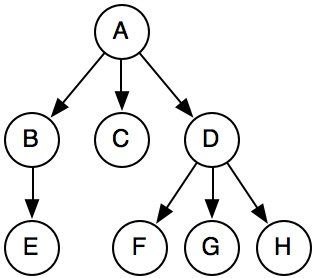
\includegraphics[width=2in]{background/media-graphs/rootedtree.jpg}
\end{center}

\begin{center}
\begin{tabular}{rcl}
root & : & $A$\\
leaves & : & $E$, $C$, $F$, $G$, and $H$\\
internal nodes & : & $A$, $B$, and $D$\\
children of $A$ & : & $B$, $C$ and $D$\\
parent of $E$ & : & $B$\\
descendants of $A$ & : & all nodes, including $A$ itself\\
ancestors of $F$ & : & $F$, $D$ and $A$\\
depth of $F$ & : & 2\\
height of $B$ & : & 1\\
height of the tree & : & 2\\
subtree rooted at $D$ & : & the rooted tree consisting of $D$, $F$, $G$ and $H$
\end{tabular}
\end{center}

\end{example}
\end{cluster}

